\section{Profil}
Durch verschiedene Optionen kann man entweder sein eigenes Profil betrachten und bearbeiten oder andere Profile anschauen.\\
Eigens Profil:\\
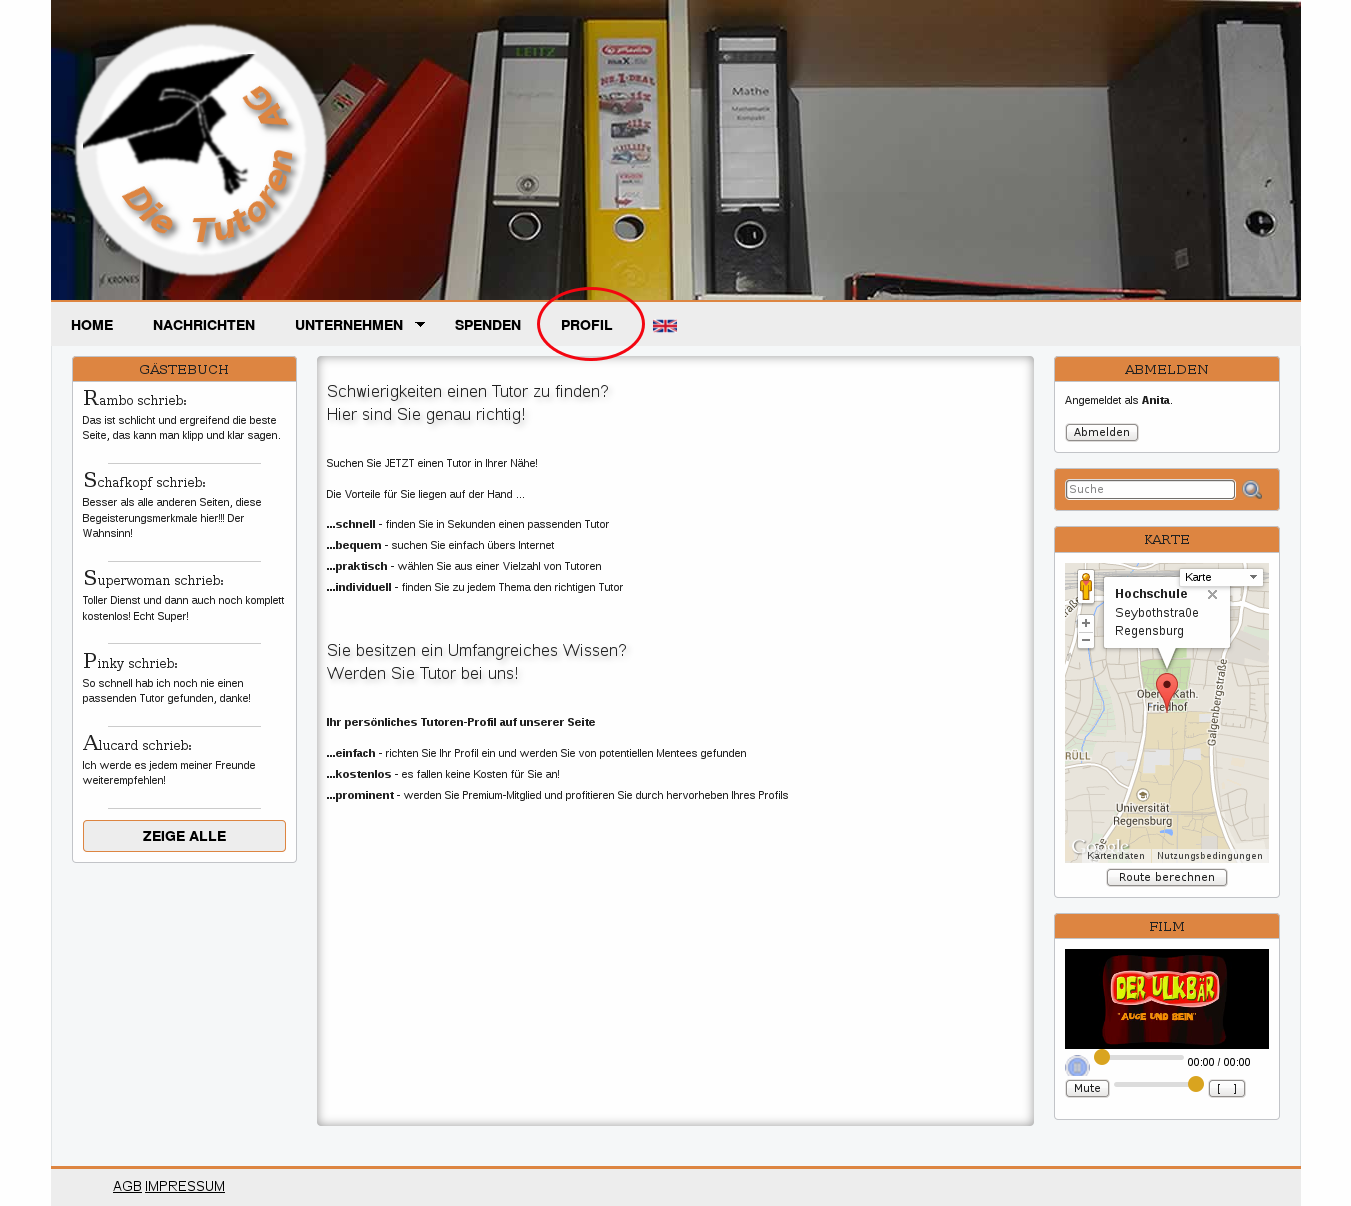
\includegraphics[width=1\textwidth]{../Screenshots/de/Startseite_profile_change}
\newpage
Andere Profile erreicht man z.B. nach der Suche und auswählen eines Namens:\\
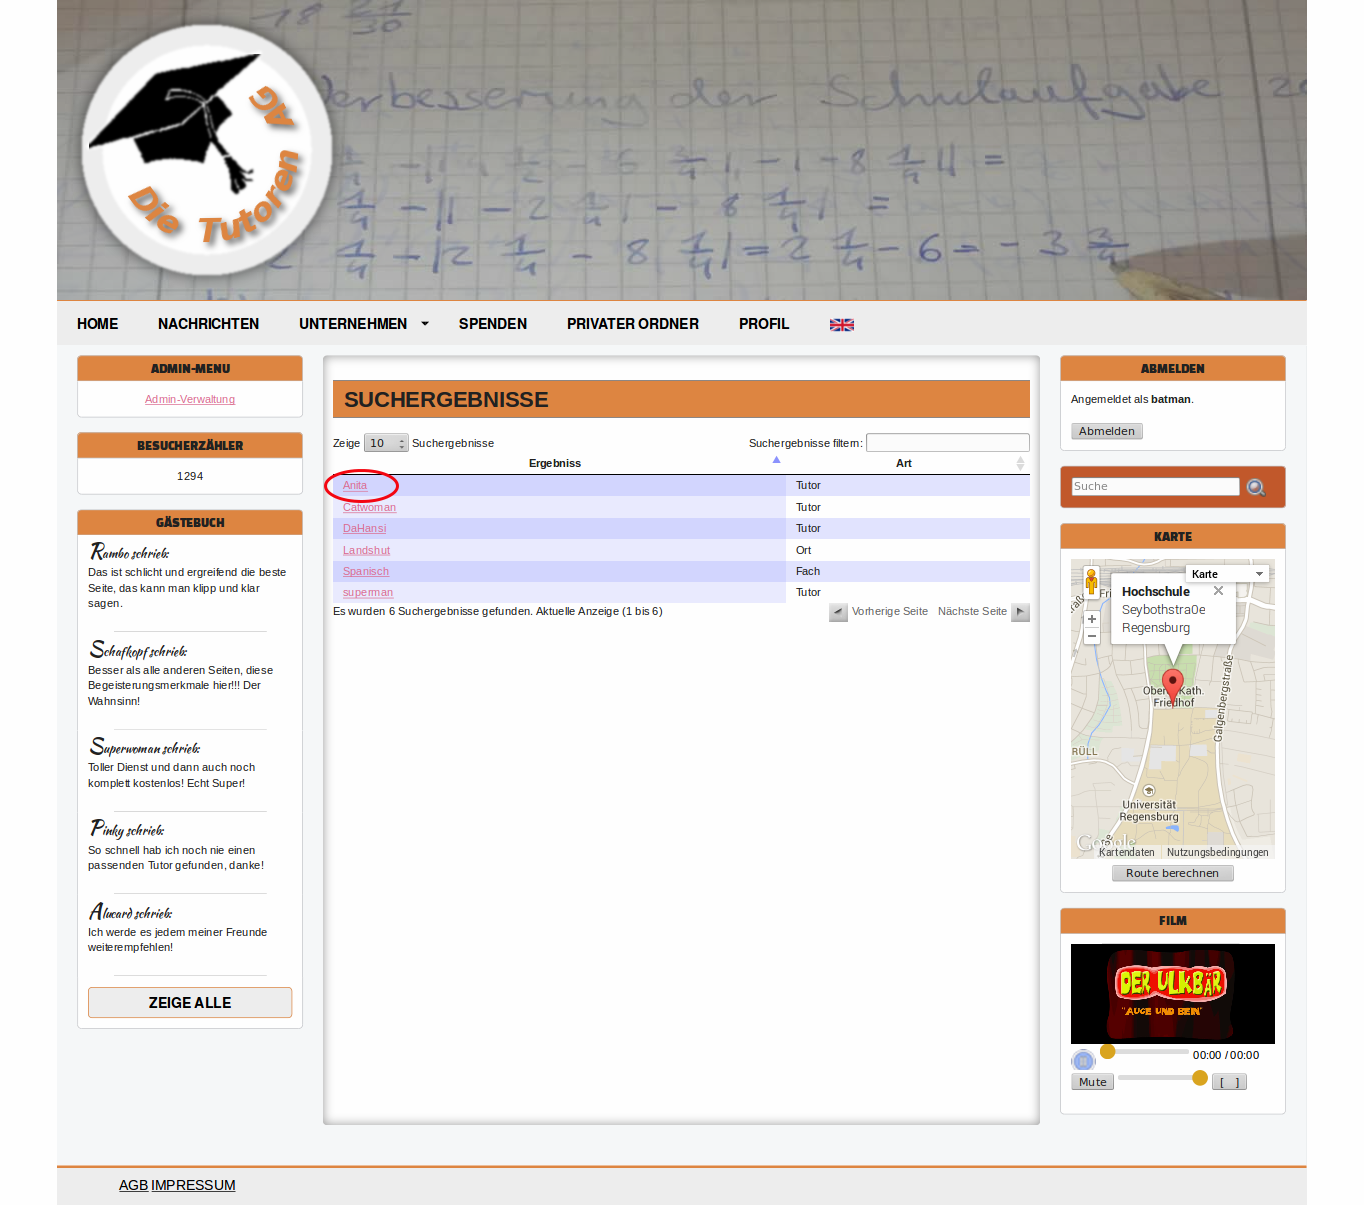
\includegraphics[width=1\textwidth]{../Screenshots/de/Suchergebnisse-profile-doku}

\newpage

\subsection{Eigenes Profil}
Im eigenen Profil kann man seine eigene Daten einsenden, und alle \underline{nicht} grau hinterlegten Daten verändern und durch Absenden des Formulars diese \\ verbindlich in der Datenbank verändern.
Darunter kann man entweder zur Tutorverwaltung gelangen oder auch sein Profil löschen.\\
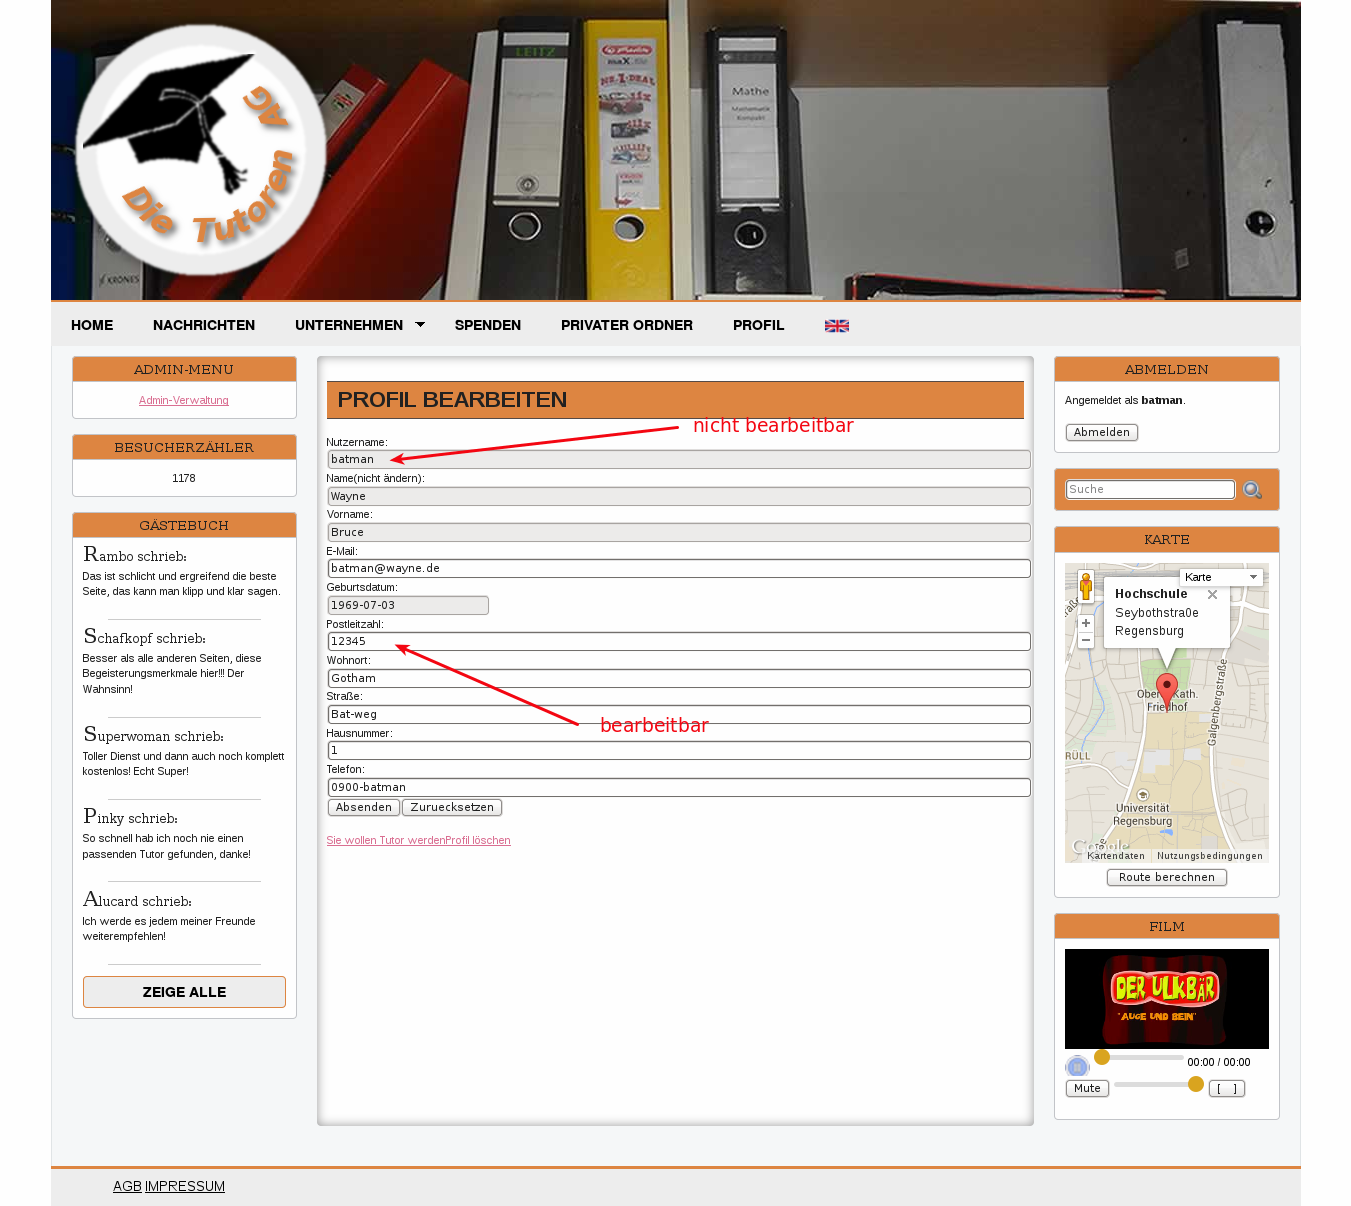
\includegraphics[width=1\textwidth]{../Screenshots/de/Profil-bearbeiten}

\newpage

\subsection{Anderes Profil}
Auf anderen Profilen kann man die Daten dieses Benutzer betrachten, Kontakt mit diesem aufnehmen und, wenn der besuchte User Tutor ist, auch die Daten über seine Tutortätigkeit einsehen.\\
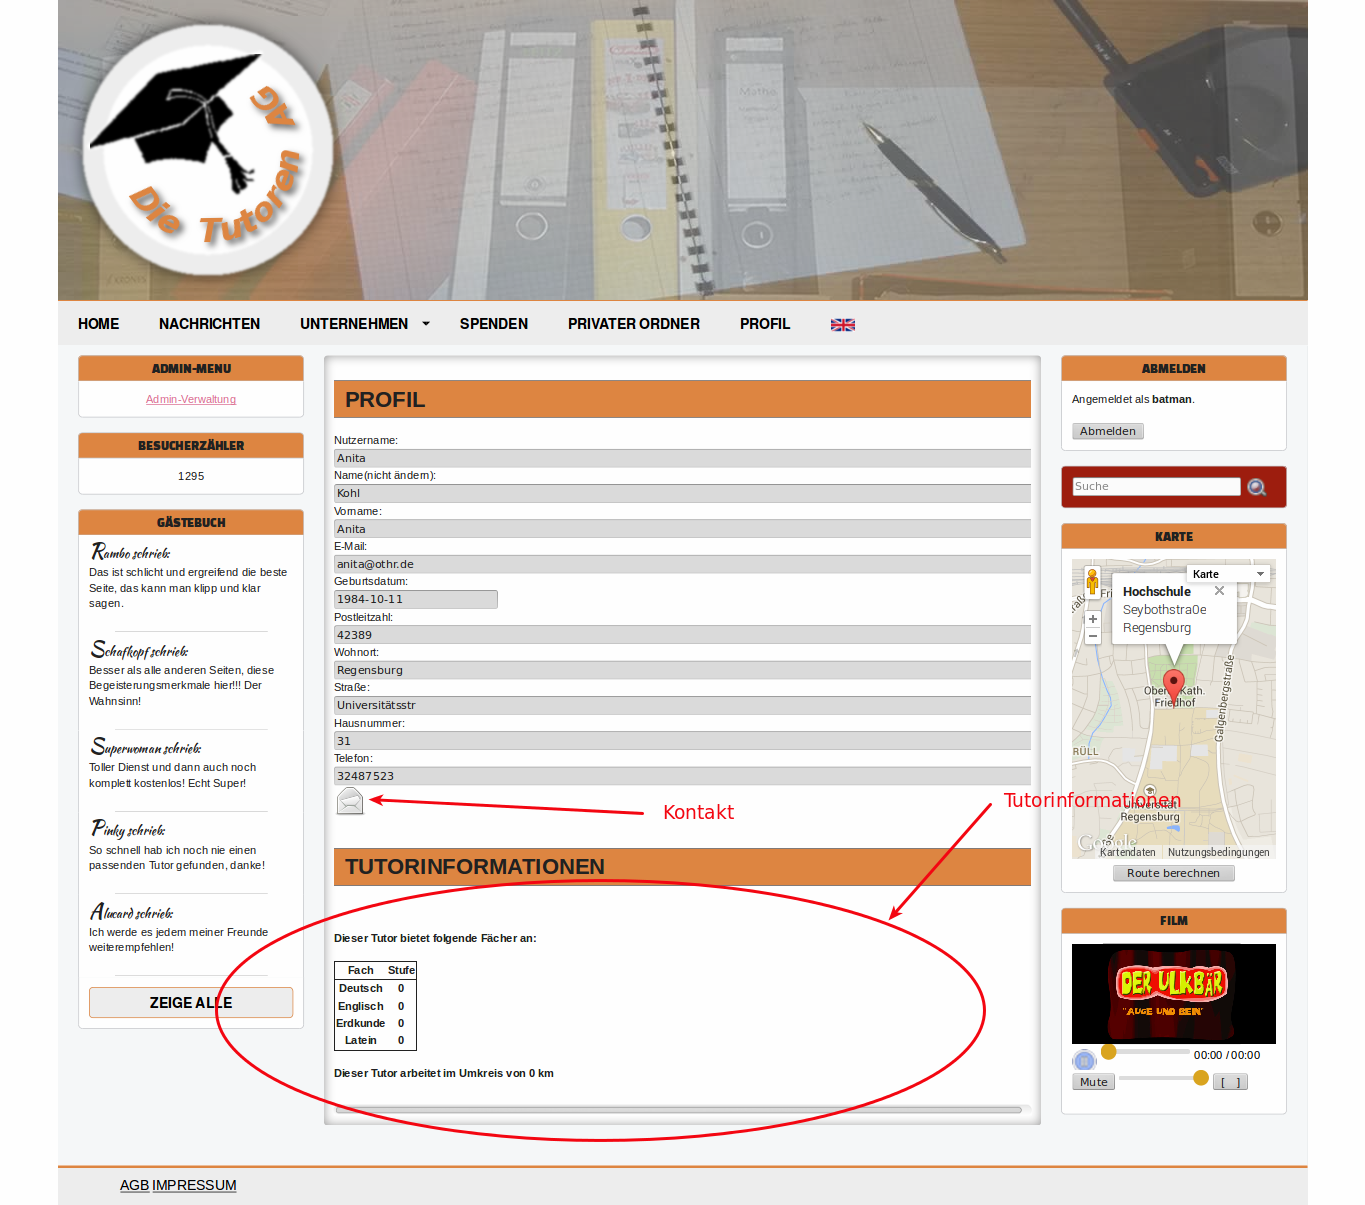
\includegraphics[width=1\textwidth]{../Screenshots/de/Profil_bearbeiten_fremdes}